% !TEX root = main.tex
% !TEX program = pdflatex
\documentclass[11pt]{article}

\usepackage[margin=1in]{geometry}
\usepackage{graphicx}
\usepackage{booktabs}
\usepackage{longtable}
\usepackage{float}
\usepackage{hyperref}
\usepackage{caption}

\hypersetup{colorlinks=true, linkcolor=blue, citecolor=blue, urlcolor=blue}

\title{Data Description}
\author{Maria Jose Perez \and Juan Manuel Lozano \and Samuel Suárez Valle}
\date{\today}

\begin{document}

\maketitle
\tableofcontents
\newpage

\section{Data and Sample}

The analysis sample comes from the 2018 GEIH, scraped in \texttt{01\_Web\_Scrapping.r} and
cleaned in \texttt{02\_Data\_Cleaning.r}, which restricts the data to employed adults
(\texttt{age >= 18} and \texttt{ocu == 1}). The outcome variable, \texttt{y\_total\_m}
(total monthly labor income), is missing for a subset of observations; \autoref{tab:balance}
compares observations with and without \texttt{y\_total\_m} to characterize this
missingness.

\begin{table}[!h]
\centering
\caption{\label{tab:balance}Balance table: missing vs. non-missing income}
\centering
\resizebox{\ifdim\width>\linewidth\linewidth\else\width\fi}{!}{
\begin{tabular}[t]{lrrrrr}
\toprule
Variable & Non-missing & Missing & Diff. & t-stat & p-value\\
\midrule
Age & 38.8882 & 43.9865 & -5.0983 & -13.7957 & 0.0000\\
Female & 0.4734 & 0.4421 & 0.0313 & 2.5095 & 0.0122\\
Male & 0.5266 & 0.5579 & -0.0313 & -2.5095 & 0.0122\\
None & 0.0066 & 0.0152 & -0.0086 & -2.8946 & 0.0038\\
Primary incomplete (1-4) & 0.0448 & 0.0602 & -0.0153 & -2.6027 & 0.0093\\
\addlinespace
Primary complete (5) & 0.0912 & 0.0922 & -0.0011 & -0.1466 & 0.8835\\
Secondary incomplete (6-10) & 0.1173 & 0.0917 & 0.0256 & 3.4938 & 0.0005\\
Secondary complete (11) & 0.3260 & 0.2655 & 0.0605 & 5.4181 & 0.0000\\
Tertiary & 0.4141 & 0.4753 & -0.0611 & -4.8805 & 0.0000\\
Private employee & 0.5931 & 0.3290 & 0.2641 & 22.2752 & 0.0000\\
\addlinespace
Government employee & 0.0387 & 0.0343 & 0.0044 & 0.9493 & 0.3426\\
Domestic worker & 0.0381 & 0.0084 & 0.0297 & 11.0735 & 0.0000\\
Self-employed & 0.2974 & 0.4021 & -0.1047 & -8.5664 & 0.0000\\
Employer & 0.0320 & 0.0861 & -0.0540 & -7.9331 & 0.0000\\
Unpaid family worker & 0.0000 & 0.1164 & -0.1164 & -15.3017 & 0.0000\\
\addlinespace
Unpaid worker (other household) & 0.0000 & 0.0231 & -0.0231 & -6.4764 & 0.0000\\
Day laborer & 0.0001 & 0.0000 & 0.0001 & 1.0000 & 0.3173\\
Other & 0.0005 & 0.0006 & 0.0000 & -0.0346 & 0.9724\\
Informal & 0.3976 & 0.5427 & -0.1452 & -11.6262 & 0.0000\\
Formal & 0.6024 & 0.4573 & 0.1452 & 11.6262 & 0.0000\\
\bottomrule
\end{tabular}}
\end{table}


\section{General Descriptive Statistics}

\autoref{tab:general-continuous} and \autoref{tab:general-categorical} summarize the
key variables for the full analysis sample: age, usual weekly hours worked, total
monthly income, sex, maximum education level, and formality.\footnote{From this
section onward, every statistic is weighted by \texttt{fex\_c} --- GEIH's
person-level expansion factor --- using the \texttt{srvyr} R package: a survey
design object is built with \texttt{as\_survey\_design(weights = fex\_c)}, and
means, standard deviations and quartiles are computed on it with
\texttt{survey\_mean()}, \texttt{survey\_sd()} and \texttt{survey\_quantile()}, so
each respondent counts as the number of population individuals they represent
rather than as a single observation. N, the minimum and the maximum are reported
unweighted, since sample size and range describe the sample itself rather than a
population quantity.}

In \autoref{tab:general-categorical}, N is likewise a weighted population-total
estimate (via \texttt{survey\_total()}) rather than a raw sample count, and \%
is that category's share of the weighted group total.

\begin{table}[H]
\centering
\caption{\label{tab:general-continuous}General descriptive statistics: continuous variables}
\centering
\resizebox{\ifdim\width>\linewidth\linewidth\else\width\fi}{!}{
\begin{tabular}[t]{lrrrrrrrr}
\toprule
Variable & N & Mean & SD & P25 & Median & P75 & Min & Max\\
\midrule
Age & 16542 & 39.23 & 13.33 & 28 & 37.0 & 49 & 18 & 9.4e+01\\
Usual weekly hours worked & 16542 & 47.19 & 15.63 & 40 & 48.0 & 50 & 1 & 1.3e+02\\
Total monthly income & 14764 & 1623821.59 & 2452556.05 & 800000 & 996119.7 & 1549807 & 84 & 7.0e+07\\
\bottomrule
\end{tabular}}
\end{table}


\begin{table}[!h]
\centering
\caption{\label{tab:general-categorical}General descriptive statistics: categorical variables}
\centering
\resizebox{\ifdim\width>\linewidth\linewidth\else\width\fi}{!}{
\begin{tabular}[t]{llrr}
\toprule
Variable & Category & N & \%\\
\midrule
sex & Female & 7775 & 47.00\\
sex & Male & 8767 & 53.00\\
maxEducLevel & None & 124 & 0.75\\
maxEducLevel & Primary incomplete (1-4) & 769 & 4.65\\
maxEducLevel & Primary complete (5) & 1510 & 9.13\\
\addlinespace
maxEducLevel & Secondary incomplete (6-10) & 1895 & 11.46\\
maxEducLevel & Secondary complete (11) & 5284 & 31.94\\
maxEducLevel & Tertiary & 6959 & 42.07\\
formal & Informal & 6835 & 41.32\\
formal & Formal & 9707 & 58.68\\
\bottomrule
\end{tabular}}
\end{table}


\section{Descriptive Statistics by Group}

These tables additionally report skewness and (non-excess) kurtosis for
income --- kurtosis of 3 corresponds to a normal distribution.\footnote{As with
the tables above, these are weighted by \texttt{fex\_c}. \texttt{srvyr} has no
built-in weighted skewness/kurtosis estimator, so these are computed directly
from \texttt{fex\_c}-weighted central moments: skewness $= m_3 / m_2^{1.5}$ and
kurtosis $= m_4 / m_2^2$, where $m_k = \sum_i w_i (x_i - \bar{x}_w)^k \big/
\sum_i w_i$ is the $k$-th weighted central moment and $\bar{x}_w$ the
weighted mean.}

\subsection{By Sex}

\begin{table}[!h]
\centering
\caption{\label{tab:by-sex-continuous}Descriptive statistics by sex: continuous variables}
\centering
\resizebox{\ifdim\width>\linewidth\linewidth\else\width\fi}{!}{
\begin{tabular}[t]{llrrrrrrrrrr}
\toprule
Sex & Variable & N & Mean & SD & Min & P25 & Median & P75 & Max & Skewness & Kurtosis\\
\midrule
Female & Age & 7775 & 39.25 & 13.03 & 18 & 28.0 & 38 & 49 & 93 & 0.43 & 2.42\\
Female & Usual weekly hours worked & 7775 & 44.00 & 15.33 & 1 & 40.0 & 48 & 48 & 126 & -0.15 & 4.73\\
Female & Total monthly income & 6989 & 1492482.83 & 2335430.74 & 84 & 700000.0 & 932743 & 1488211 & 70000000 & 10.10 & 200.95\\
Male & Age & 8767 & 39.60 & 13.87 & 18 & 28.0 & 37 & 50 & 94 & 0.48 & 2.42\\
Male & Usual weekly hours worked & 8767 & 49.67 & 15.25 & 1 & 45.0 & 48 & 55 & 130 & 0.41 & 5.67\\
\addlinespace
Male & Total monthly income & 7775 & 1729974.70 & 2509229.46 & 97 & 803857.7 & 1040000 & 1625000 & 50000000 & 7.34 & 87.83\\
\bottomrule
\end{tabular}}
\end{table}


\begin{table}[H]
\centering
\caption{\label{tab:by-sex-categorical}Descriptive statistics by sex: categorical variables}
\centering
\resizebox{\ifdim\width>\linewidth\linewidth\else\width\fi}{!}{
\begin{tabular}[t]{lllrr}
\toprule
Variable & Sex & Category & N & \%\\
\midrule
formal & Female & Informal & 800222 & 41.69\\
formal & Female & Formal & 1119338 & 58.31\\
formal & Male & Informal & 903873 & 41.07\\
formal & Male & Formal & 1296881 & 58.93\\
\bottomrule
\end{tabular}}
\end{table}


\subsection{By Age Range}

\begin{table}[!h]
\centering
\caption{\label{tab:by-age-continuous}Descriptive statistics by age range: continuous variables}
\centering
\resizebox{\ifdim\width>\linewidth\linewidth\else\width\fi}{!}{
\begin{tabular}[t]{llrrrrrrrrrr}
\toprule
Age range & Variable & N & Mean & SD & Min & P25 & Median & P75 & Max & Skewness & Kurtosis\\
\midrule
18-28 & Usual weekly hours worked & 4324 & 46.49 & 14.87 & 1 & 40 & 48 & 48 & 119 & -0.19 & 5.32\\
18-28 & Total monthly income & 3984 & 1180455.47 & 1128411.10 & 15000 & 800000 & 934453 & 1288211 & 30000000 & 9.15 & 164.66\\
29-38 & Usual weekly hours worked & 4311 & 48.68 & 14.14 & 1 & 45 & 48 & 50 & 130 & 0.42 & 6.29\\
29-38 & Total monthly income & 3964 & 1728634.06 & 2132998.14 & 5000 & 869453 & 1093211 & 1843294 & 70000000 & 10.89 & 280.53\\
39-50 & Usual weekly hours worked & 4035 & 48.36 & 15.14 & 2 & 40 & 48 & 50 & 130 & 0.53 & 6.04\\
\addlinespace
39-50 & Total monthly income & 3573 & 1952791.88 & 3118978.46 & 30000 & 800000 & 1000000 & 1900000 & 60100000 & 7.09 & 83.50\\
51-94 & Usual weekly hours worked & 3872 & 44.31 & 17.64 & 1 & 40 & 48 & 50 & 126 & 0.07 & 3.87\\
51-94 & Total monthly income & 3243 & 1649383.42 & 2949466.53 & 84 & 500000 & 900000 & 1500000 & 50000000 & 6.32 & 62.32\\
\bottomrule
\end{tabular}}
\end{table}



\begin{longtable}[t]{lllrr}
\caption{\label{tab:by-age-categorical}Descriptive statistics by age range: categorical variables}\\
\toprule
Variable & Age range & Category & N & \%\\
\midrule
\endfirsthead
\caption[]{Descriptive statistics by age range: categorical variables \textit{(continued)}}\\
\toprule
Variable & Age range & Category & N & \%\\
\midrule
\endhead

\endfoot
\bottomrule
\endlastfoot
sex & 18-28 & Female & 1985 & 45.91\\
sex & 18-28 & Male & 2339 & 54.09\\
sex & 29-38 & Female & 2063 & 47.85\\
sex & 29-38 & Male & 2248 & 52.15\\
sex & 39-50 & Female & 1997 & 49.49\\
\addlinespace
sex & 39-50 & Male & 2038 & 50.51\\
sex & 51-94 & Female & 1730 & 44.68\\
sex & 51-94 & Male & 2142 & 55.32\\
maxEducLevel & 18-28 & None & 10 & 0.23\\
maxEducLevel & 18-28 & Primary incomplete (1-4) & 35 & 0.81\\
\addlinespace
maxEducLevel & 18-28 & Primary complete (5) & 82 & 1.90\\
maxEducLevel & 18-28 & Secondary incomplete (6-10) & 331 & 7.65\\
maxEducLevel & 18-28 & Secondary complete (11) & 1668 & 38.58\\
maxEducLevel & 18-28 & Tertiary & 2198 & 50.83\\
maxEducLevel & 29-38 & None & 15 & 0.35\\
\addlinespace
maxEducLevel & 29-38 & Primary incomplete (1-4) & 94 & 2.18\\
maxEducLevel & 29-38 & Primary complete (5) & 238 & 5.52\\
maxEducLevel & 29-38 & Secondary incomplete (6-10) & 372 & 8.63\\
maxEducLevel & 29-38 & Secondary complete (11) & 1511 & 35.06\\
maxEducLevel & 29-38 & Tertiary & 2080 & 48.26\\
\addlinespace
maxEducLevel & 39-50 & None & 25 & 0.62\\
maxEducLevel & 39-50 & Primary incomplete (1-4) & 213 & 5.28\\
maxEducLevel & 39-50 & Primary complete (5) & 465 & 11.52\\
maxEducLevel & 39-50 & Secondary incomplete (6-10) & 529 & 13.11\\
maxEducLevel & 39-50 & Secondary complete (11) & 1240 & 30.73\\
\addlinespace
maxEducLevel & 39-50 & Tertiary & 1563 & 38.74\\
maxEducLevel & 51-94 & None & 74 & 1.91\\
maxEducLevel & 51-94 & Primary incomplete (1-4) & 427 & 11.03\\
maxEducLevel & 51-94 & Primary complete (5) & 725 & 18.72\\
maxEducLevel & 51-94 & Secondary incomplete (6-10) & 663 & 17.12\\
\addlinespace
maxEducLevel & 51-94 & Secondary complete (11) & 865 & 22.34\\
maxEducLevel & 51-94 & Tertiary & 1118 & 28.87\\
formal & 18-28 & Informal & 1729 & 39.99\\
formal & 18-28 & Formal & 2595 & 60.01\\
formal & 29-38 & Informal & 1429 & 33.15\\
\addlinespace
formal & 29-38 & Formal & 2882 & 66.85\\
formal & 39-50 & Informal & 1595 & 39.53\\
formal & 39-50 & Formal & 2440 & 60.47\\
formal & 51-94 & Informal & 2082 & 53.77\\
formal & 51-94 & Formal & 1790 & 46.23\\*
\end{longtable}


\subsection{By Formality}

\begin{table}[!h]
\centering
\caption{\label{tab:by-formal-continuous}Descriptive statistics by formality: continuous variables}
\centering
\resizebox{\ifdim\width>\linewidth\linewidth\else\width\fi}{!}{
\begin{tabular}[t]{llrrrrrrrrrr}
\toprule
Formality & Variable & N & Mean & SD & Min & P25 & Median & P75 & Max & Skewness & Kurtosis\\
\midrule
Informal & Age & 6835 & 41.31 & 14.83 & 18 & 28.0 & 40 & 53 & 94 & 0.26 & 2.16\\
Informal & Usual weekly hours worked & 6835 & 45.62 & 19.91 & 1 & 35.0 & 48 & 60 & 126 & 0.12 & 3.27\\
Informal & Total monthly income & 5870 & 850156.17 & 1013723.44 & 84 & 400000.0 & 781000 & 1000000 & 28000000 & 11.20 & 211.83\\
Formal & Age & 9707 & 38.11 & 12.27 & 18 & 28.0 & 36 & 47 & 90 & 0.57 & 2.61\\
Formal & Usual weekly hours worked & 9707 & 47.99 & 11.41 & 1 & 45.0 & 48 & 48 & 130 & 0.63 & 9.32\\
\addlinespace
Formal & Total monthly income & 8894 & 2124027.34 & 2913715.33 & 8000 & 934556.5 & 1211544 & 2075917 & 70000000 & 7.43 & 100.24\\
\bottomrule
\end{tabular}}
\end{table}


\begin{table}[!h]
\centering
\caption{\label{tab:by-formal-categorical}Descriptive statistics by formality: categorical variables}
\centering
\resizebox{\ifdim\width>\linewidth\linewidth\else\width\fi}{!}{
\begin{tabular}[t]{lllrr}
\toprule
Variable & Formality & Category & N & \%\\
\midrule
sex & Informal & Female & 3230 & 47.26\\
sex & Informal & Male & 3605 & 52.74\\
sex & Formal & Female & 4545 & 46.82\\
sex & Formal & Male & 5162 & 53.18\\
maxEducLevel & Informal & None & 102 & 1.49\\
\addlinespace
maxEducLevel & Informal & Primary incomplete (1-4) & 576 & 8.43\\
maxEducLevel & Informal & Primary complete (5) & 969 & 14.18\\
maxEducLevel & Informal & Secondary incomplete (6-10) & 1244 & 18.20\\
maxEducLevel & Informal & Secondary complete (11) & 2375 & 34.75\\
maxEducLevel & Informal & Tertiary & 1569 & 22.96\\
\addlinespace
maxEducLevel & Formal & None & 22 & 0.23\\
maxEducLevel & Formal & Primary incomplete (1-4) & 193 & 1.99\\
maxEducLevel & Formal & Primary complete (5) & 541 & 5.57\\
maxEducLevel & Formal & Secondary incomplete (6-10) & 651 & 6.71\\
maxEducLevel & Formal & Secondary complete (11) & 2909 & 29.97\\
\addlinespace
maxEducLevel & Formal & Tertiary & 5390 & 55.53\\
\bottomrule
\end{tabular}}
\end{table}


\section{Income Distribution by Group}

Each figure below overlays the log-income distribution of a group (semi-transparent)
on top of the overall sample distribution (``Total''), with a dashed vertical line at
each group's mean.\footnote{Both the histogram (via ggplot2's \texttt{weight}
aesthetic) and each group's mean (a weighted mean) are weighted by
\texttt{fex\_c}, consistent with the tables above.}

\begin{figure}[H]
  \centering
  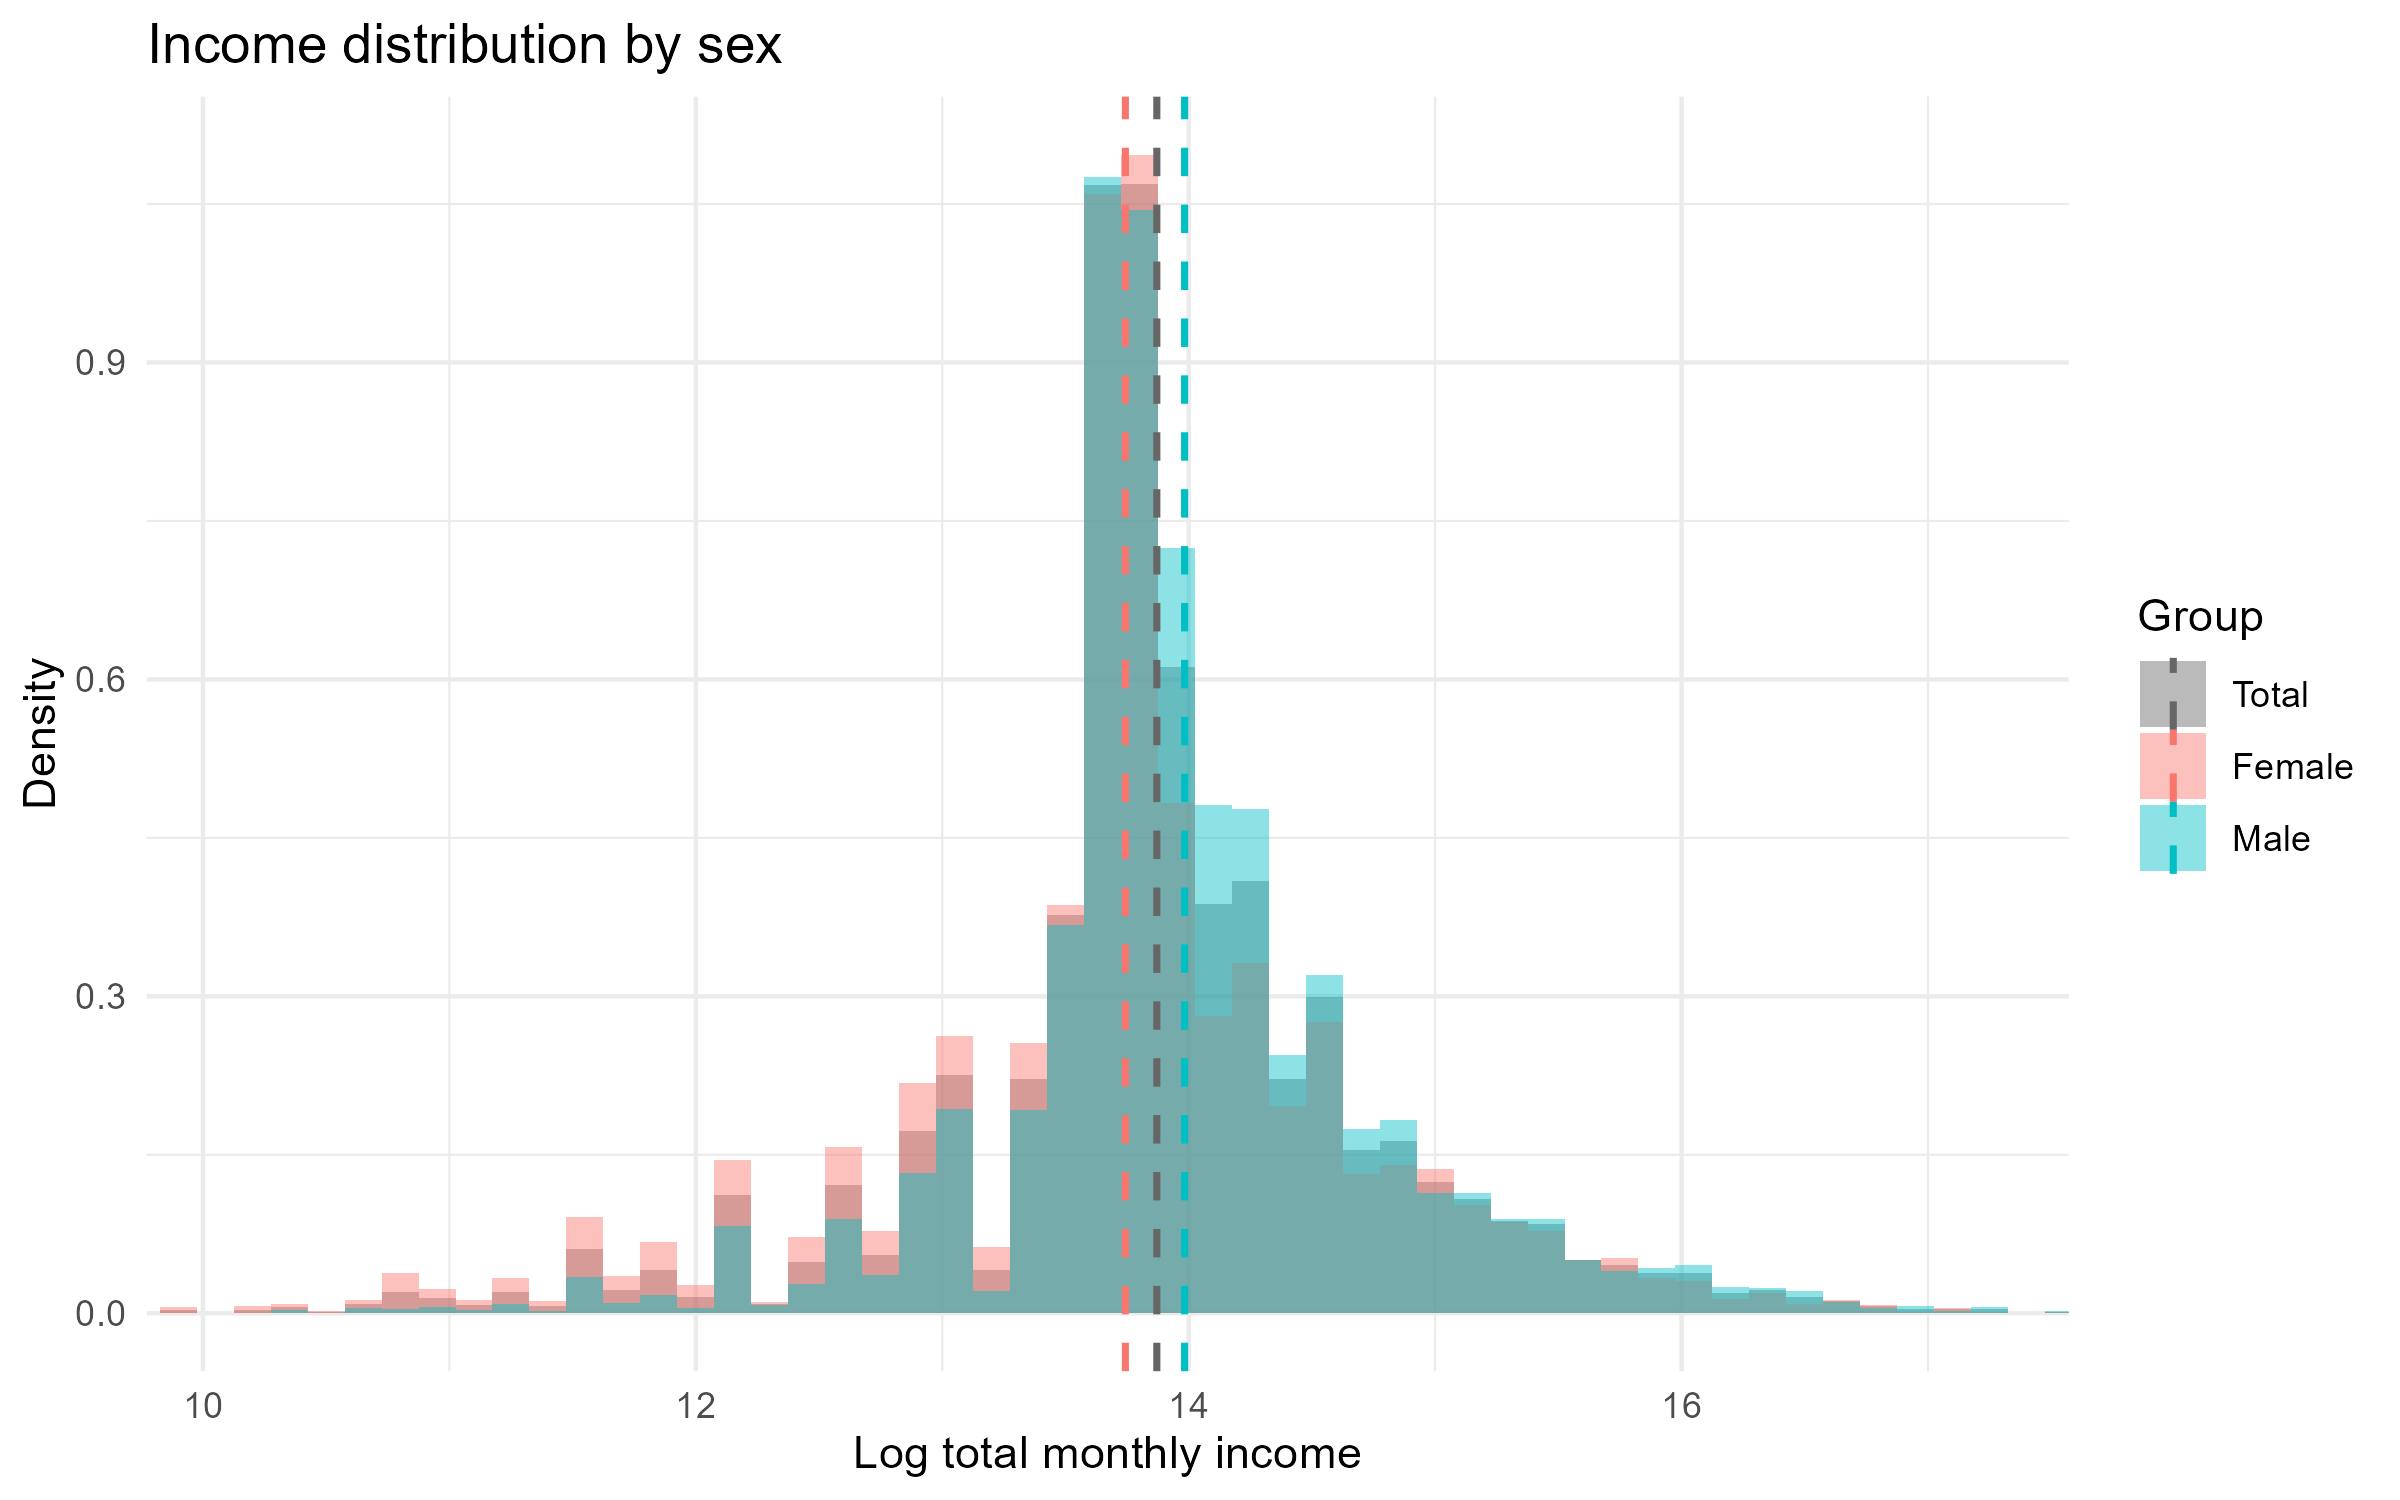
\includegraphics[width=0.85\textwidth]{../output/figures/income_dist_sex.png}
  \caption{Income distribution by sex}
\end{figure}

\begin{figure}[H]
  \centering
  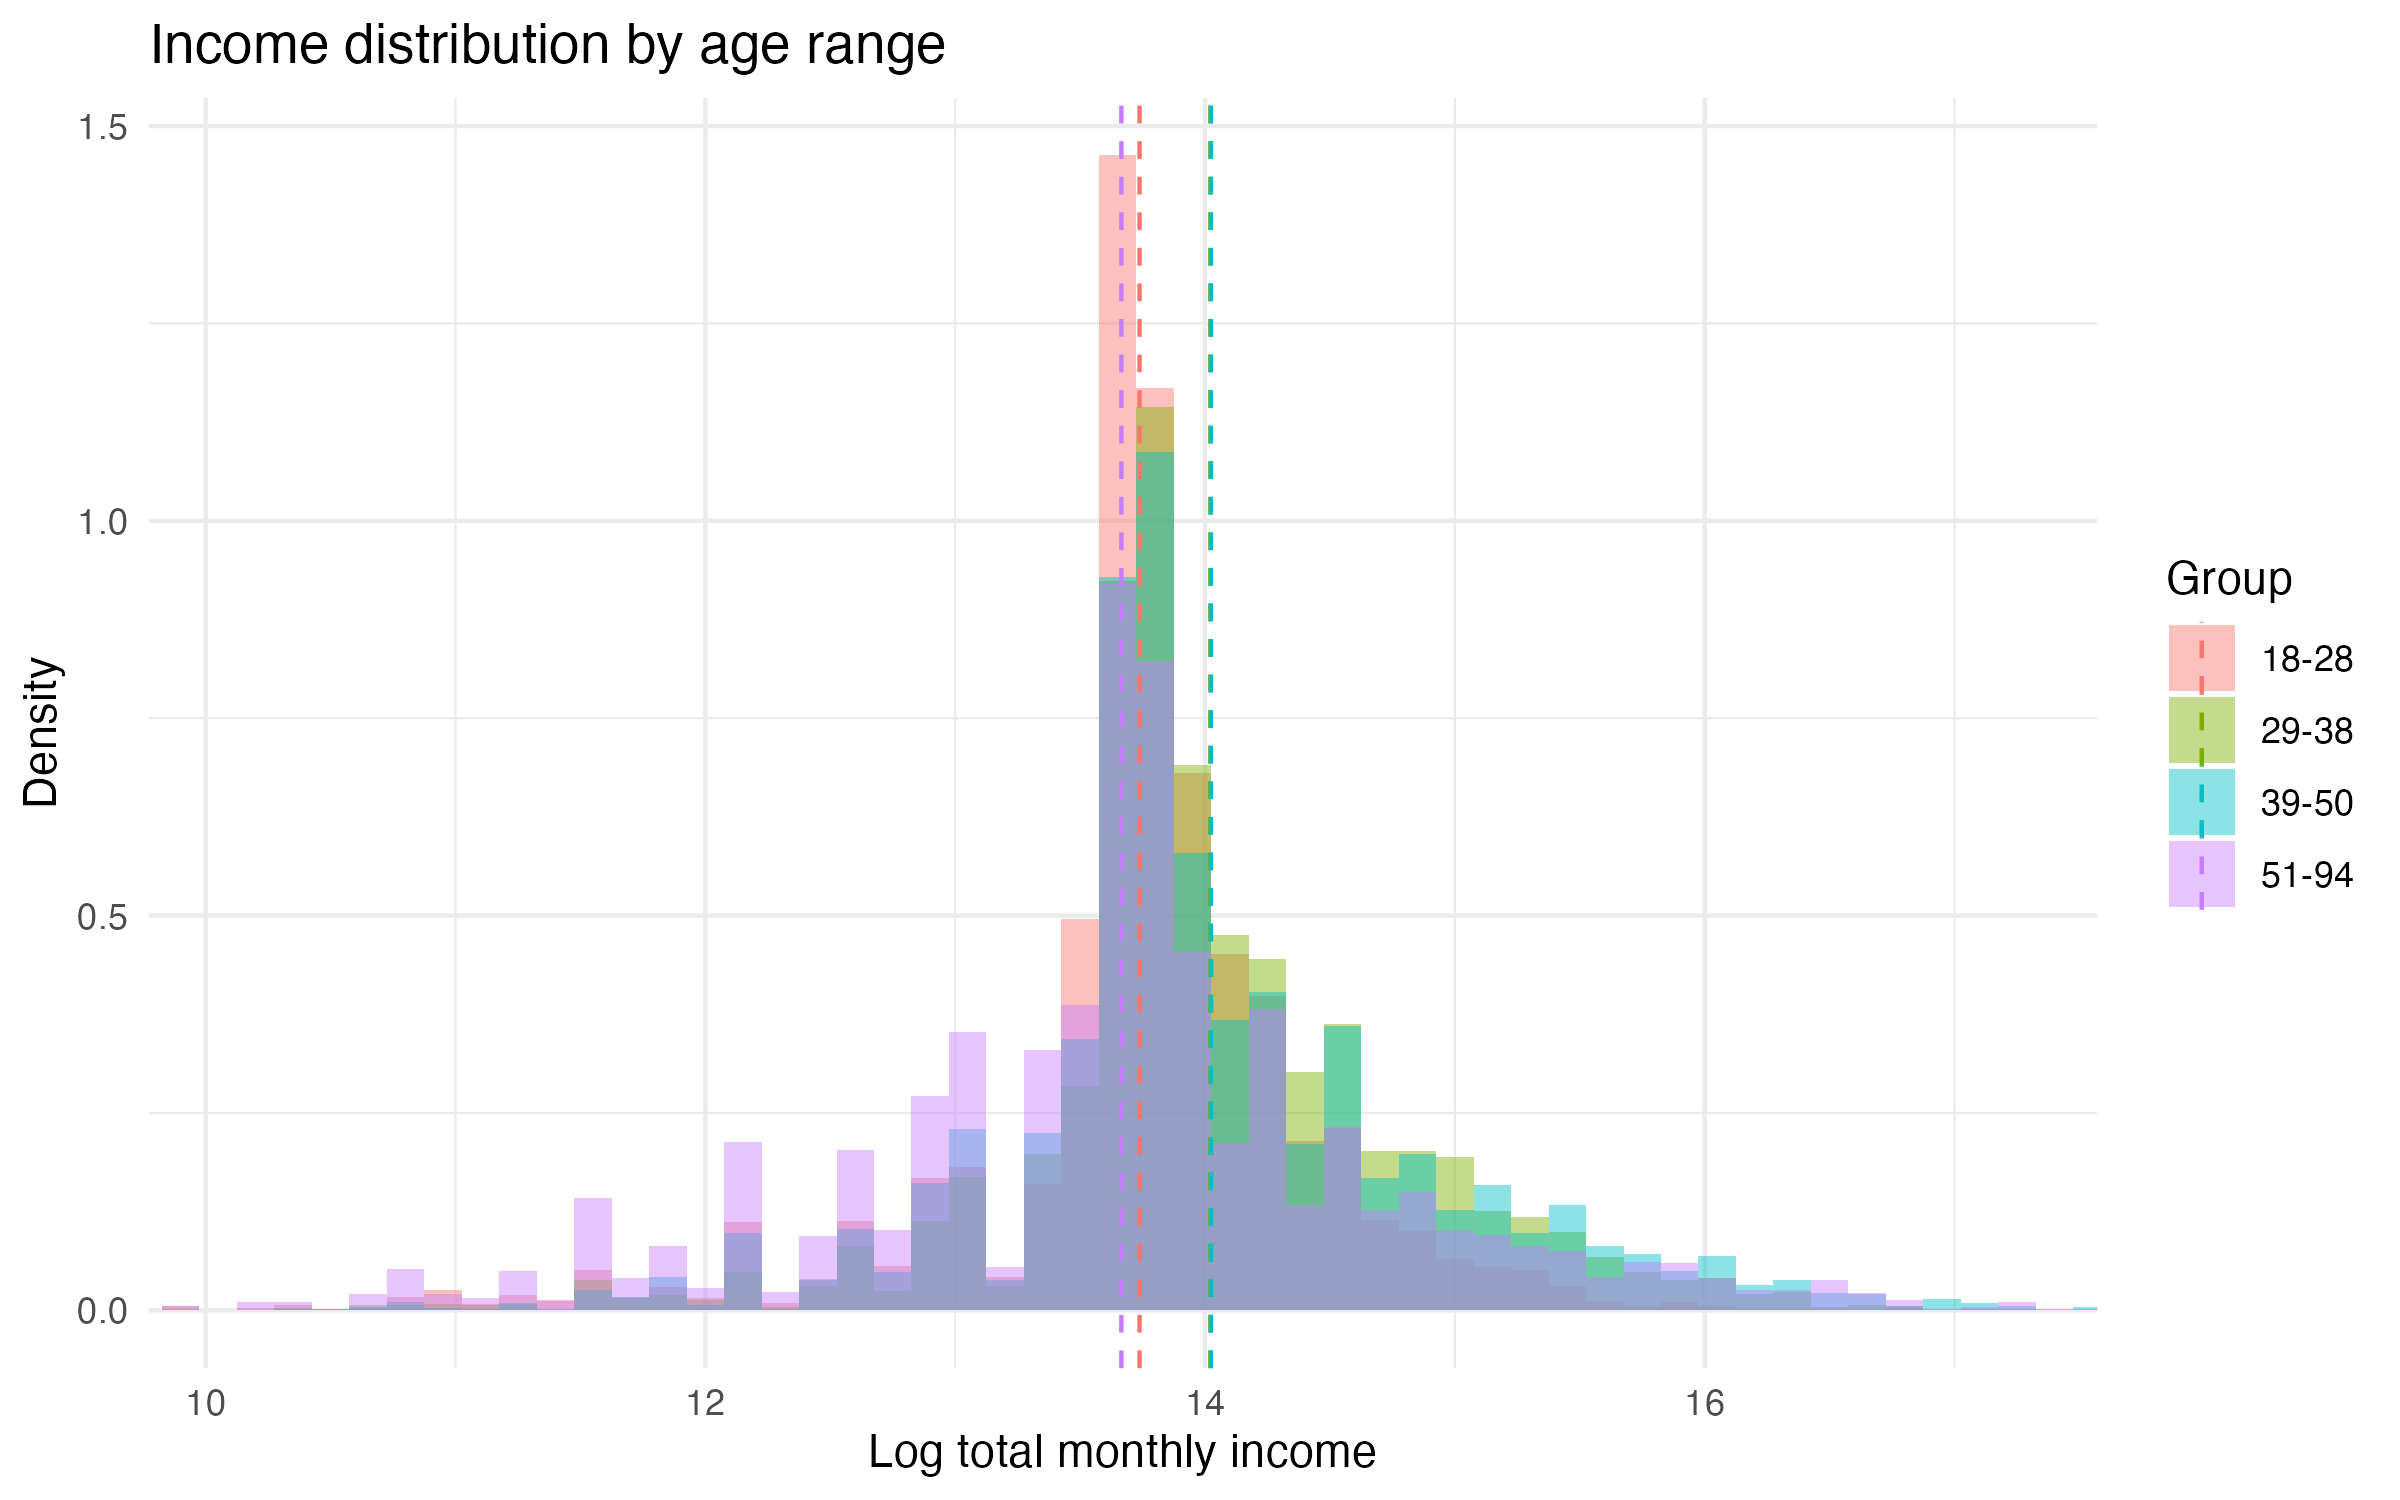
\includegraphics[width=0.85\textwidth]{../output/figures/income_dist_age.png}
  \caption{Income distribution by age range}
\end{figure}

\begin{figure}[H]
  \centering
  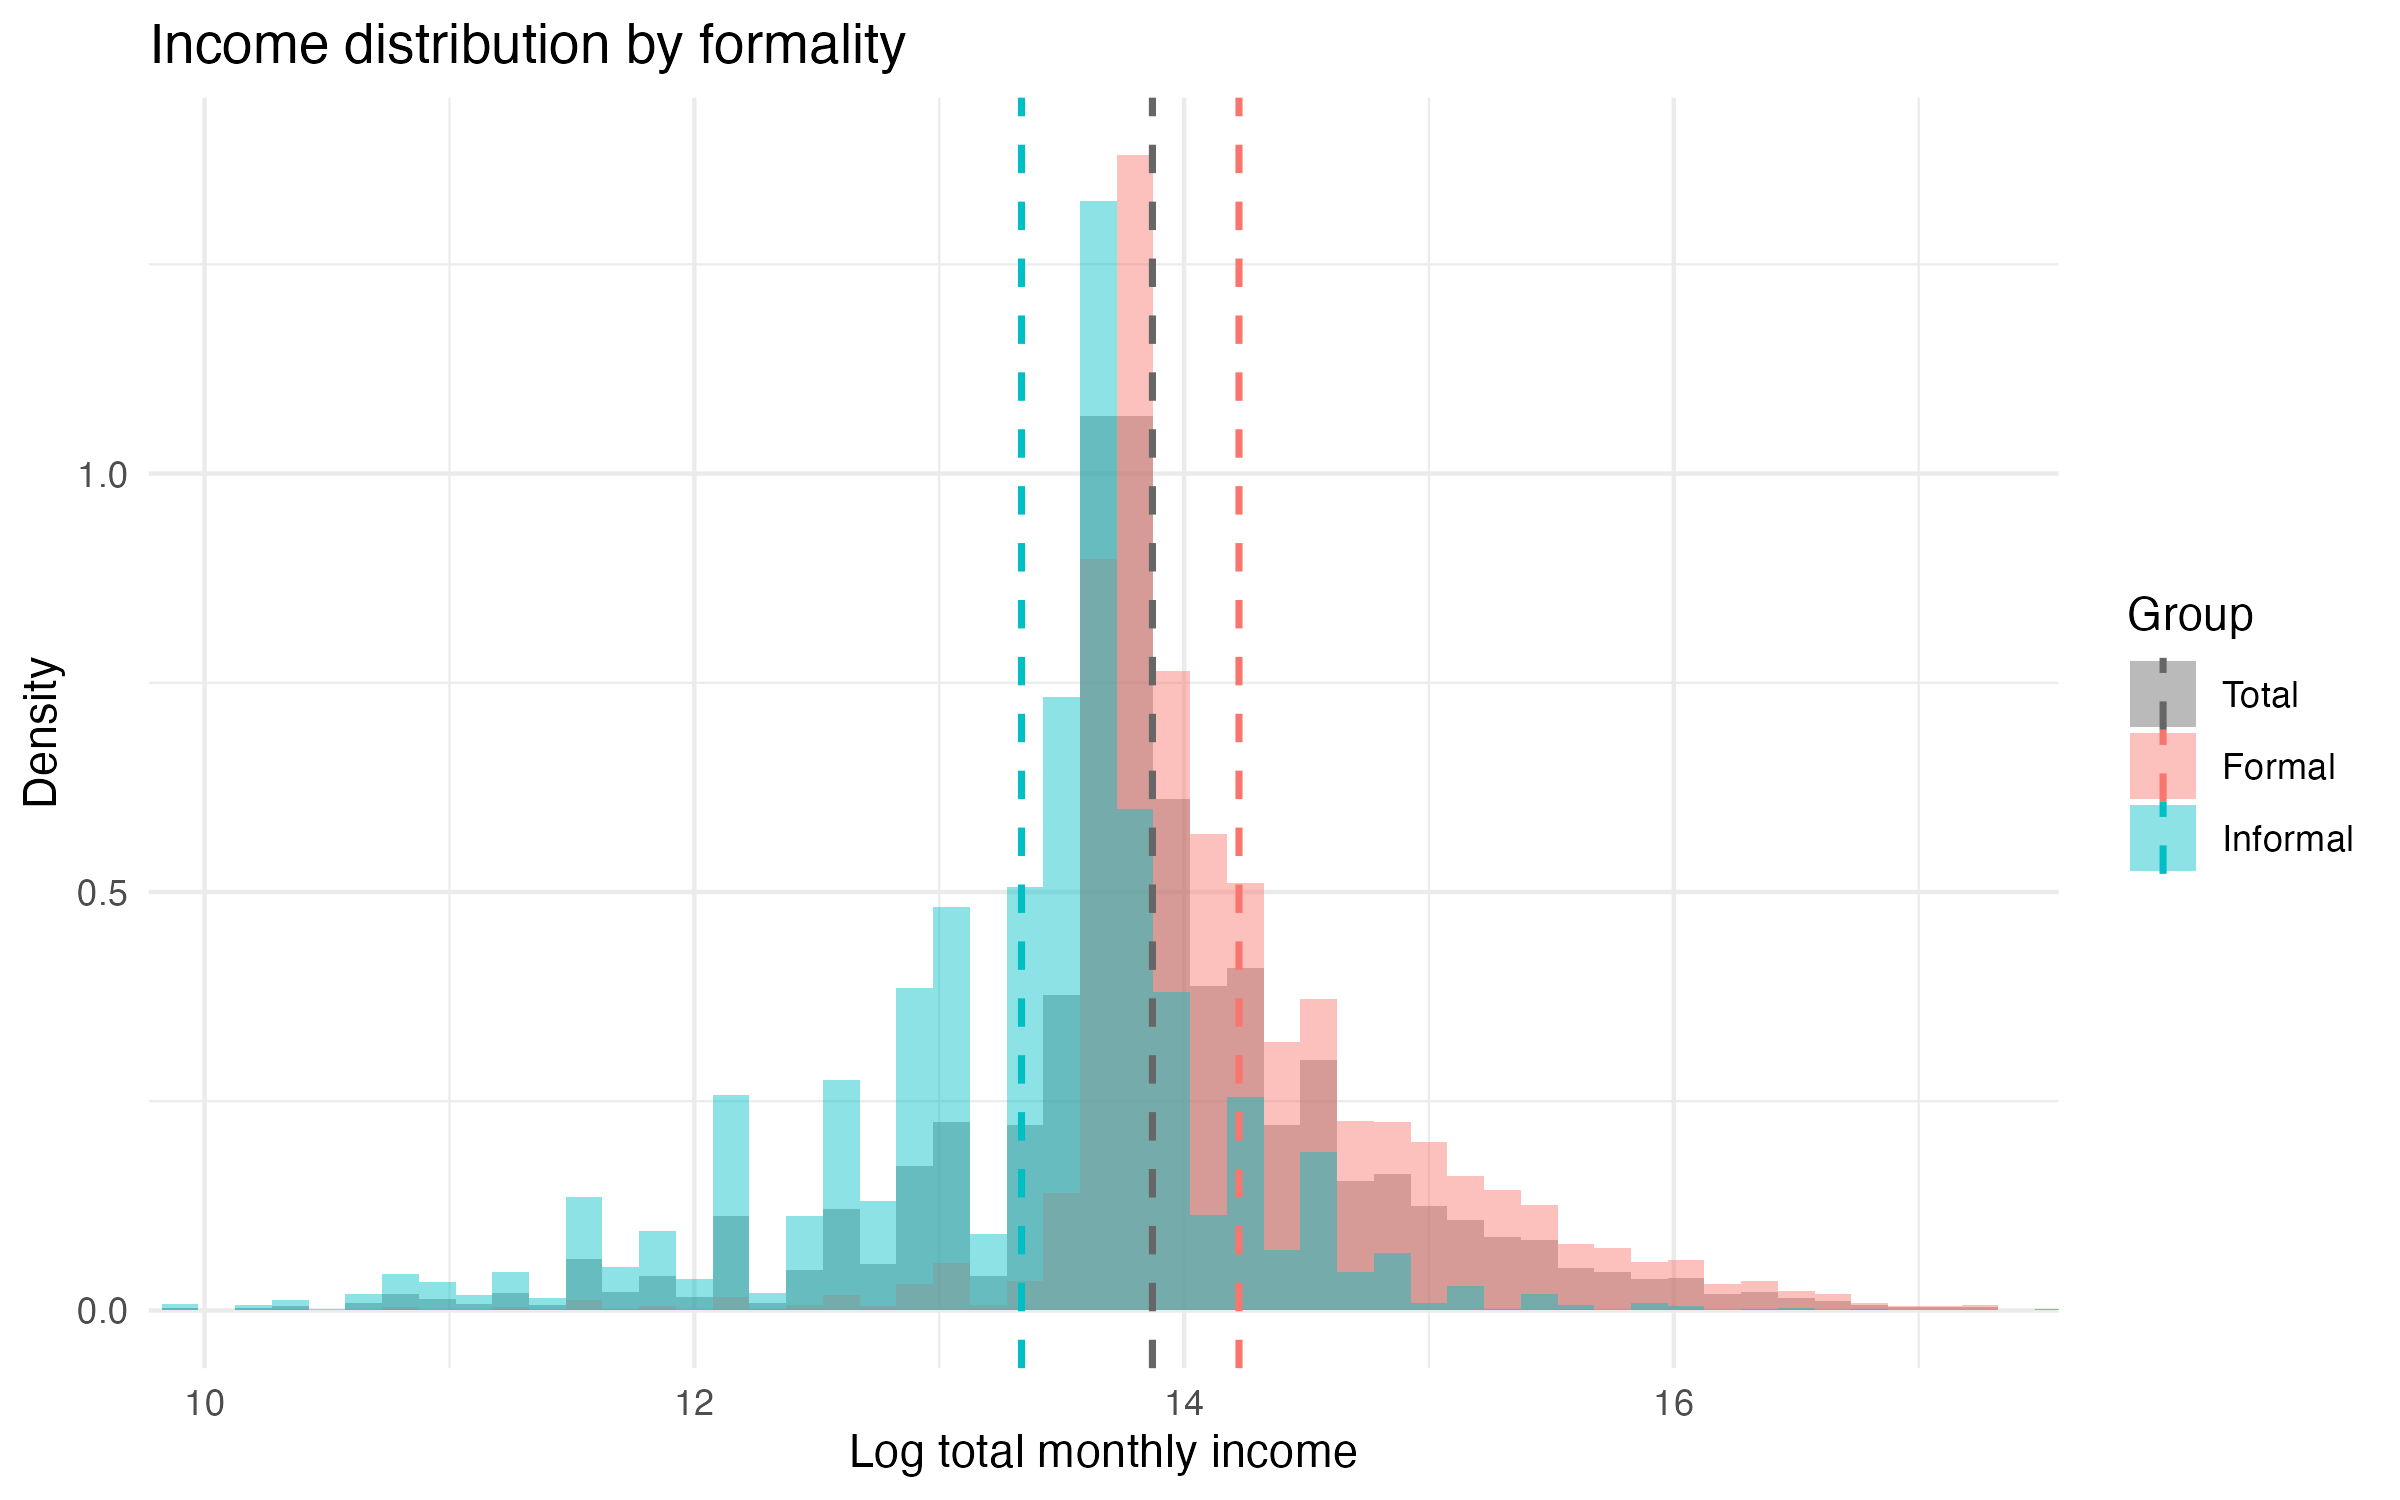
\includegraphics[width=0.85\textwidth]{../output/figures/income_dist_formal.png}
  \caption{Income distribution by formality}
\end{figure}

\section{Income vs. Age by Group}

Each figure below plots log total monthly income against age, with a separate
fitted straight line for each group.\footnote{The fitted line is a weighted
least squares regression, using \texttt{fex\_c} as the regression weight via
ggplot2's \texttt{weight} aesthetic (\texttt{geom\_smooth(aes(weight =
fex\_c), method = "lm")}).}

\begin{figure}[H]
  \centering
  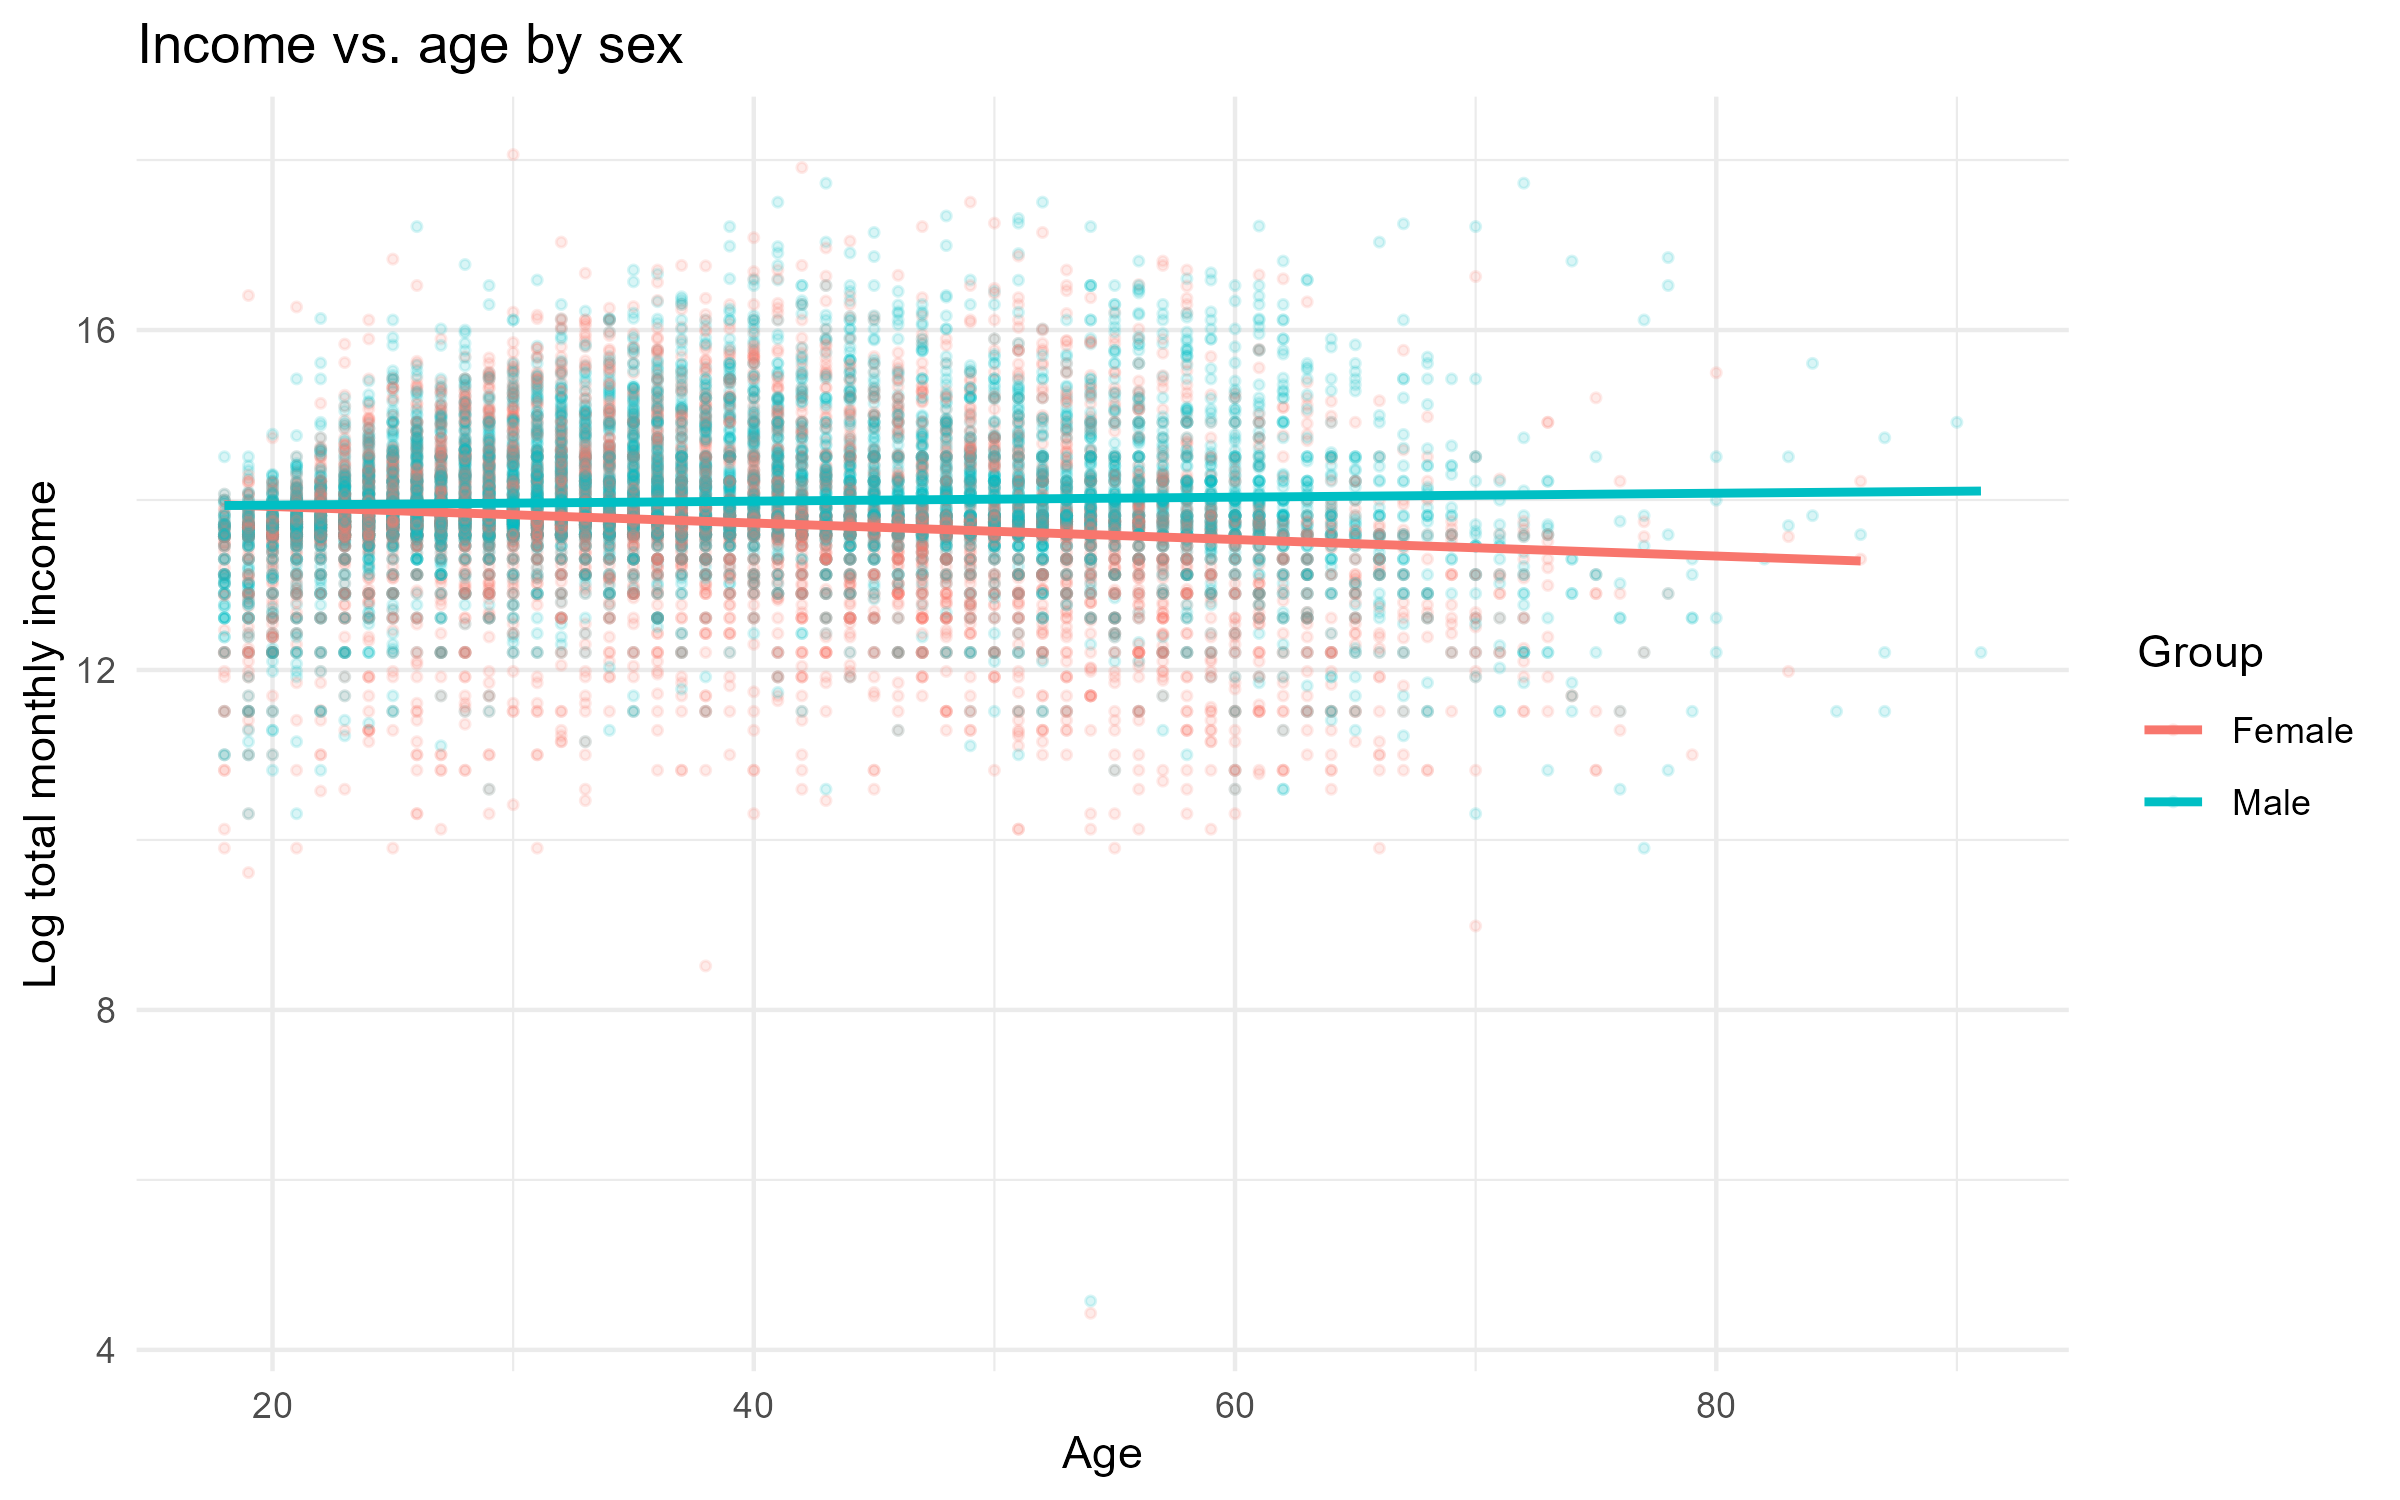
\includegraphics[width=0.85\textwidth]{../output/figures/scatter_income_age_sex.png}
  \caption{Income vs. age by sex}
\end{figure}

\begin{figure}[H]
  \centering
  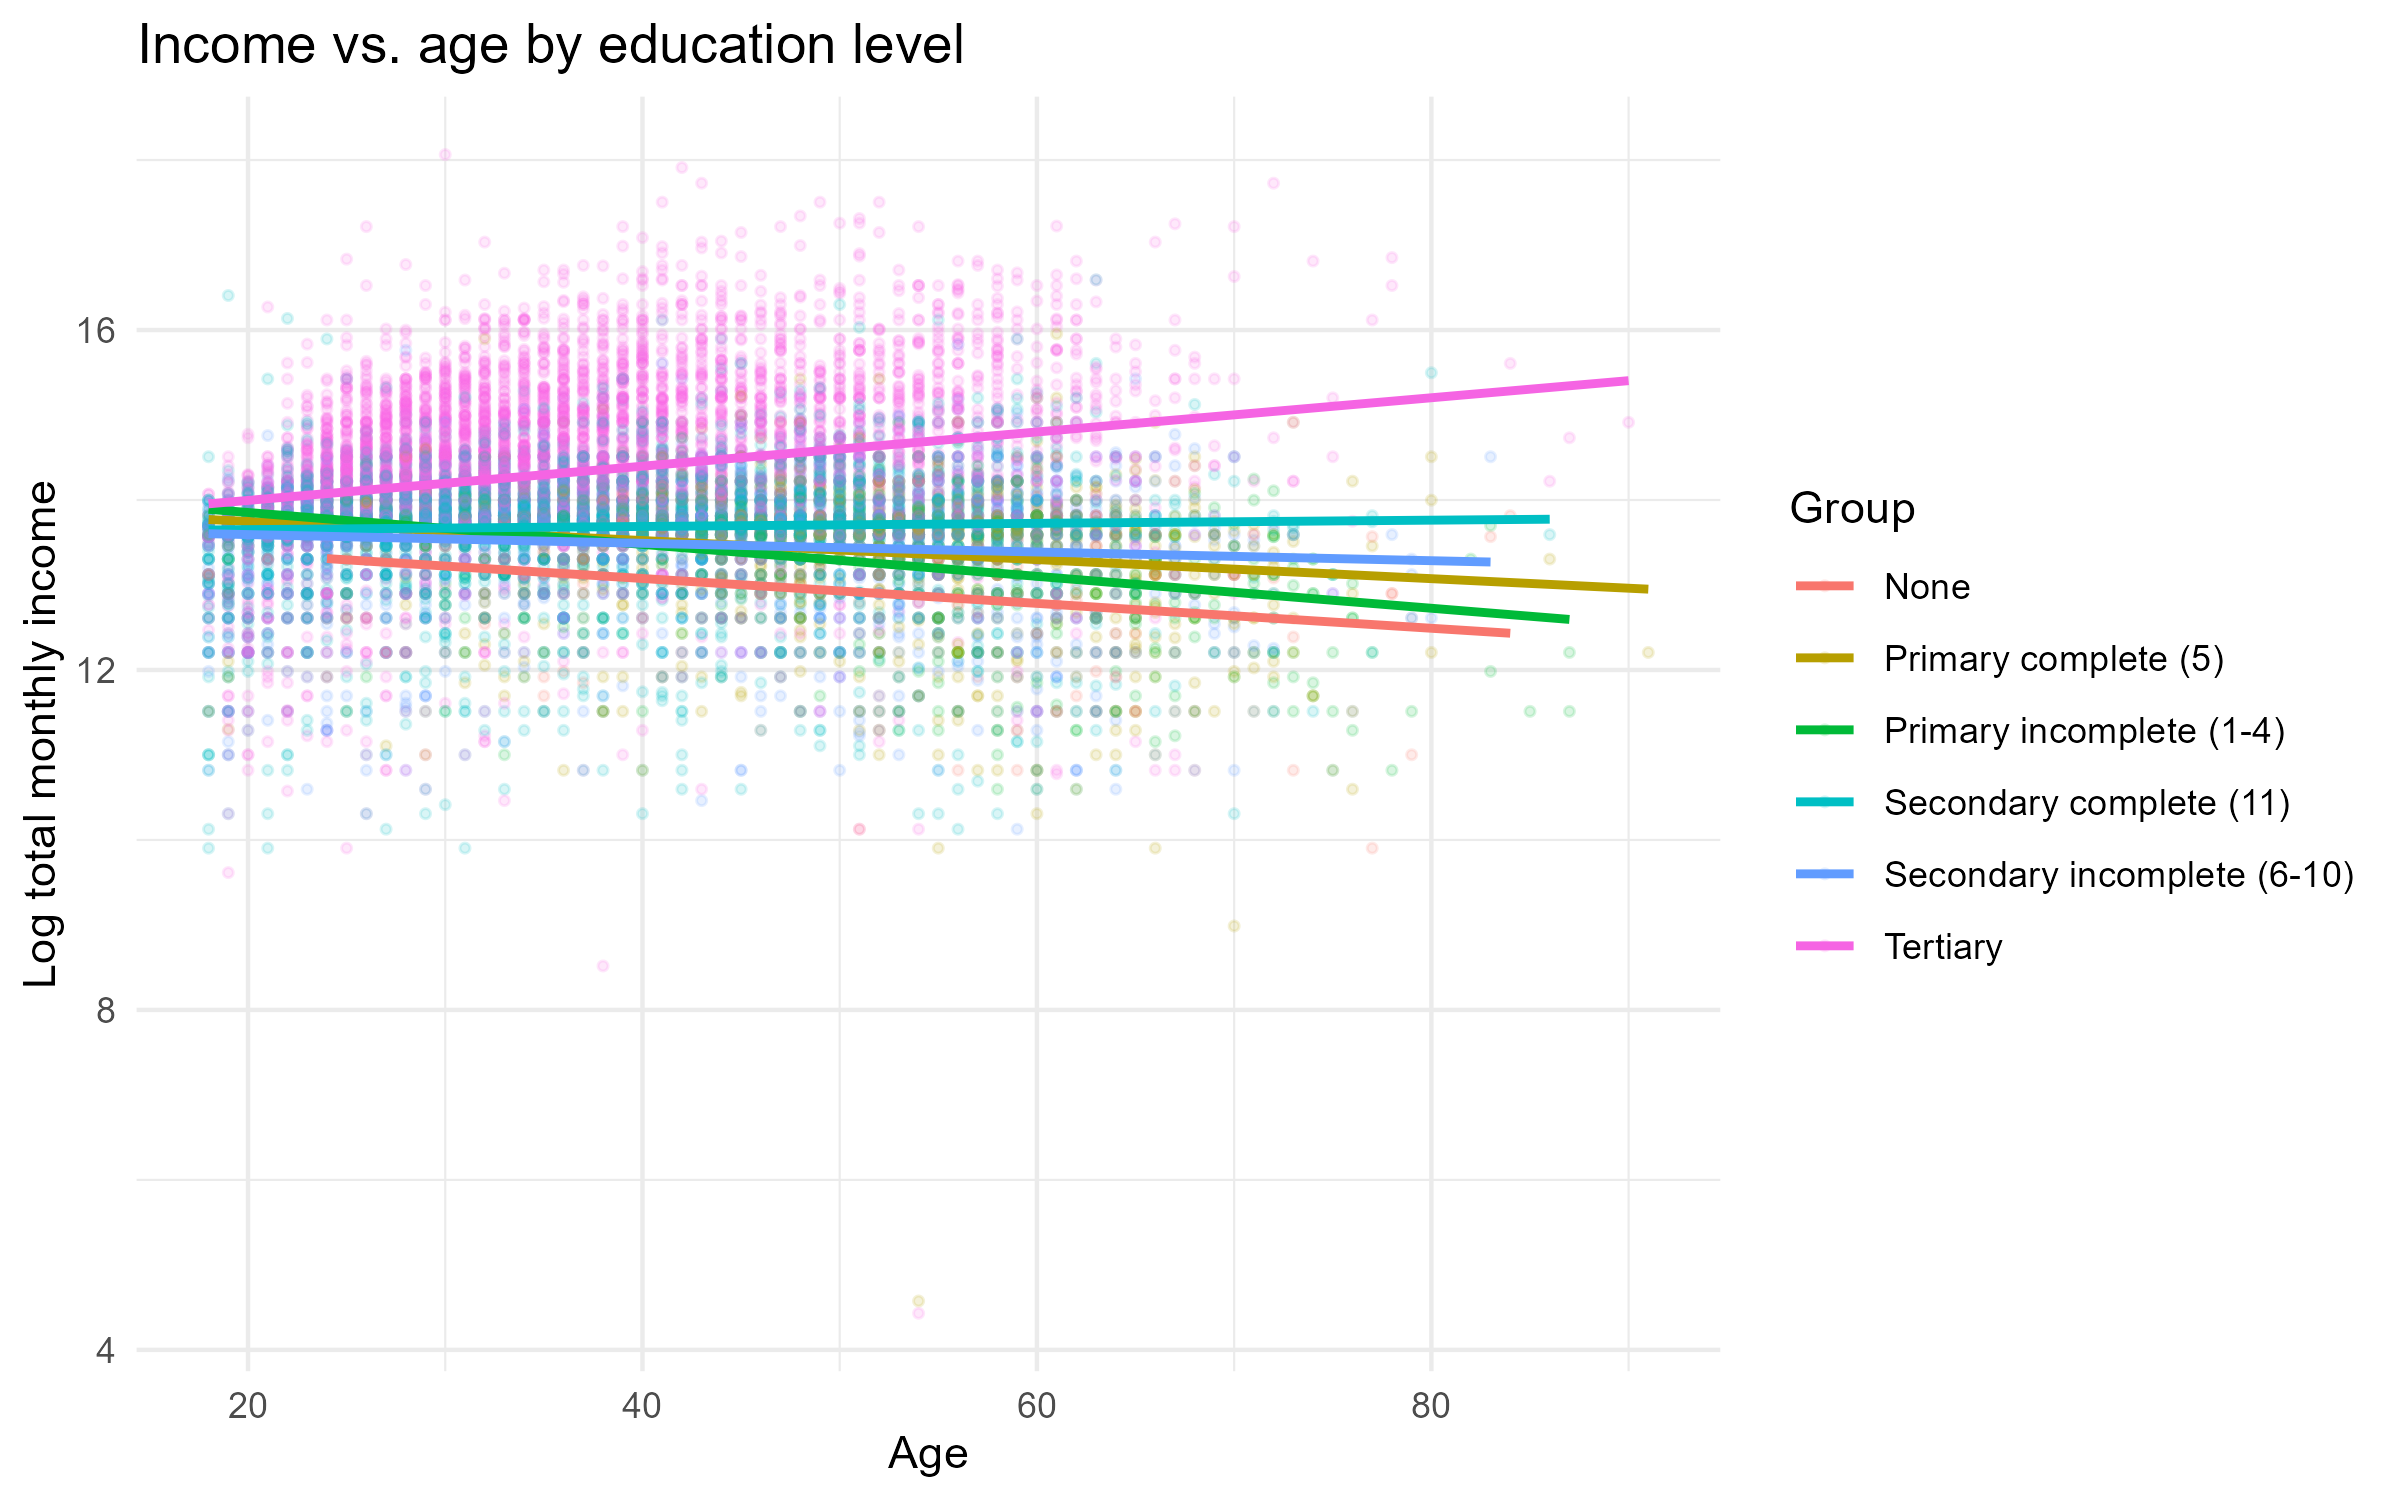
\includegraphics[width=0.85\textwidth]{../output/figures/scatter_income_age_educ.png}
  \caption{Income vs. age by education level}
\end{figure}

\begin{figure}[H]
  \centering
  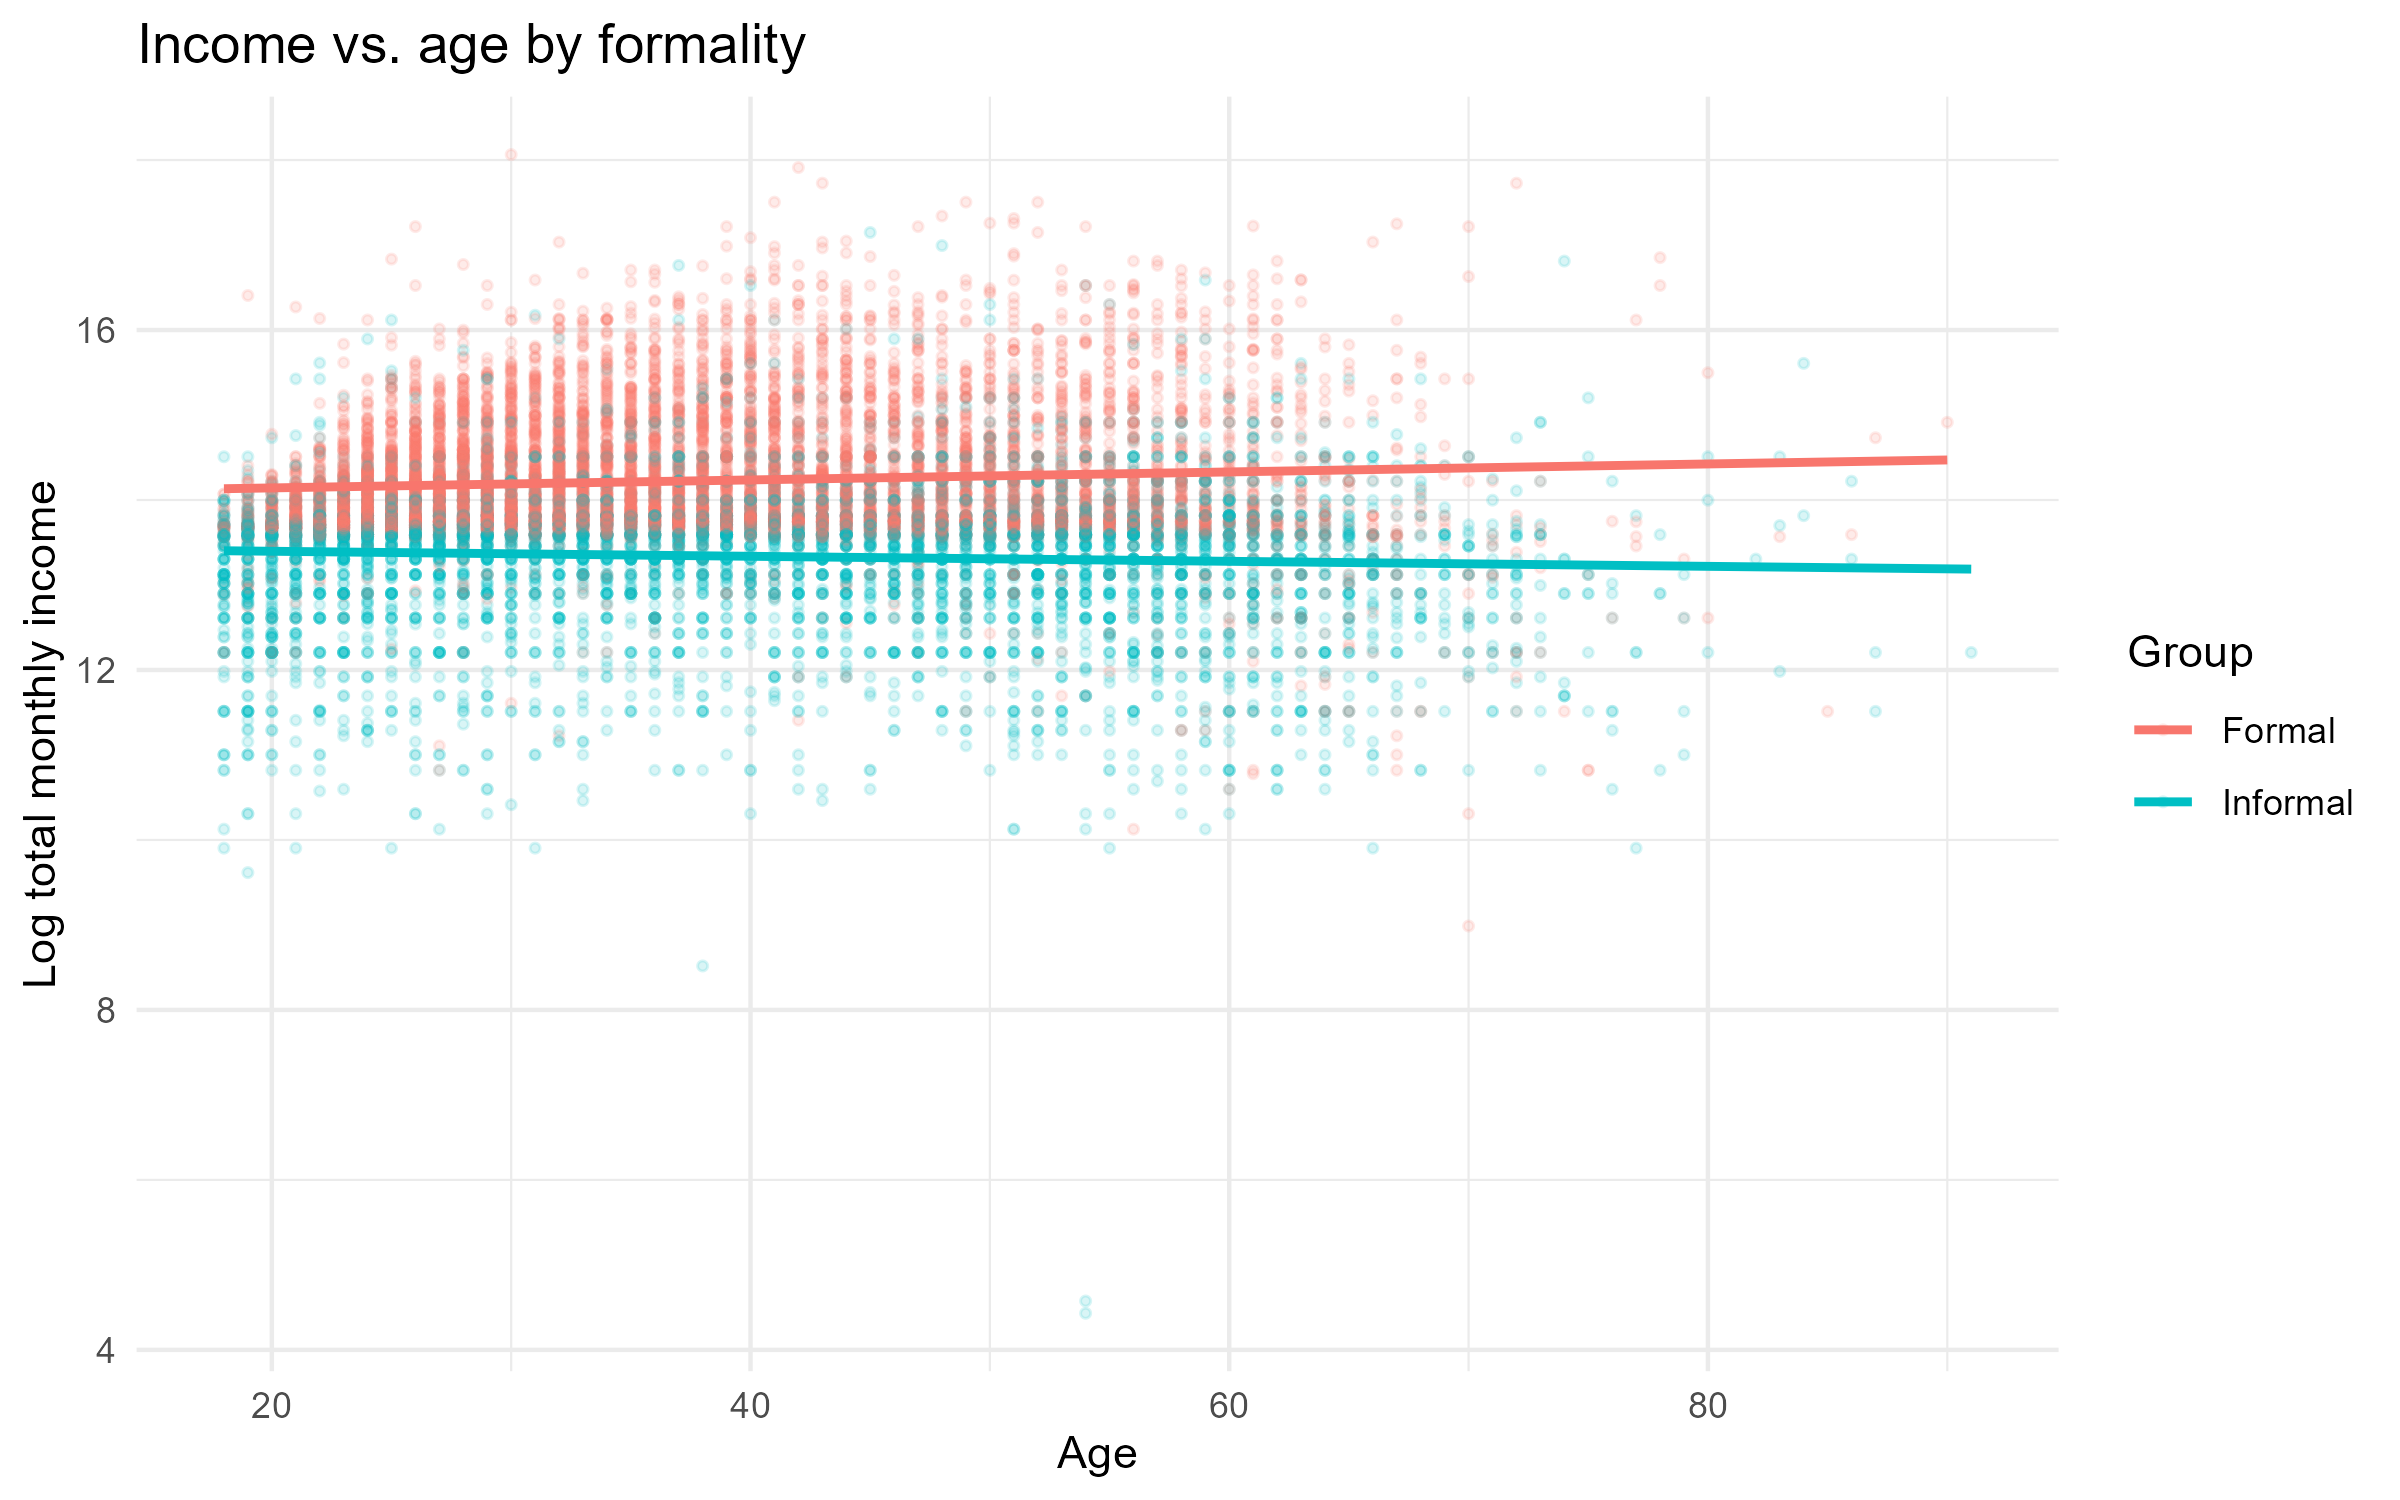
\includegraphics[width=0.85\textwidth]{../output/figures/scatter_income_age_formal.png}
  \caption{Income vs. age by formality}
\end{figure}

\end{document}
